\chapterpage{Requirements Analysis and Specification}
\mychapter{Requirements Analysis and Specification}
\label{chap:requirements}

This chapter documents the requirements used to design and implement the proposed system. It captures the elicitation and recording of the requirements, lists the functional and non-functional requirements that resulted from the elicitation and recording process, and describes the expected use of the system by a set of use cases and representative scenarios.

\section{Elicitation and Documentation of Requirements}

Requirements were gathered through a mixture of techniques suitable for an research project. The process followed is shown in Figure~\ref{fig:elicitation}, from the first application of the techniques to the establishment of a validated requirements baseline.

\begin{figure}[H]
    \centering
    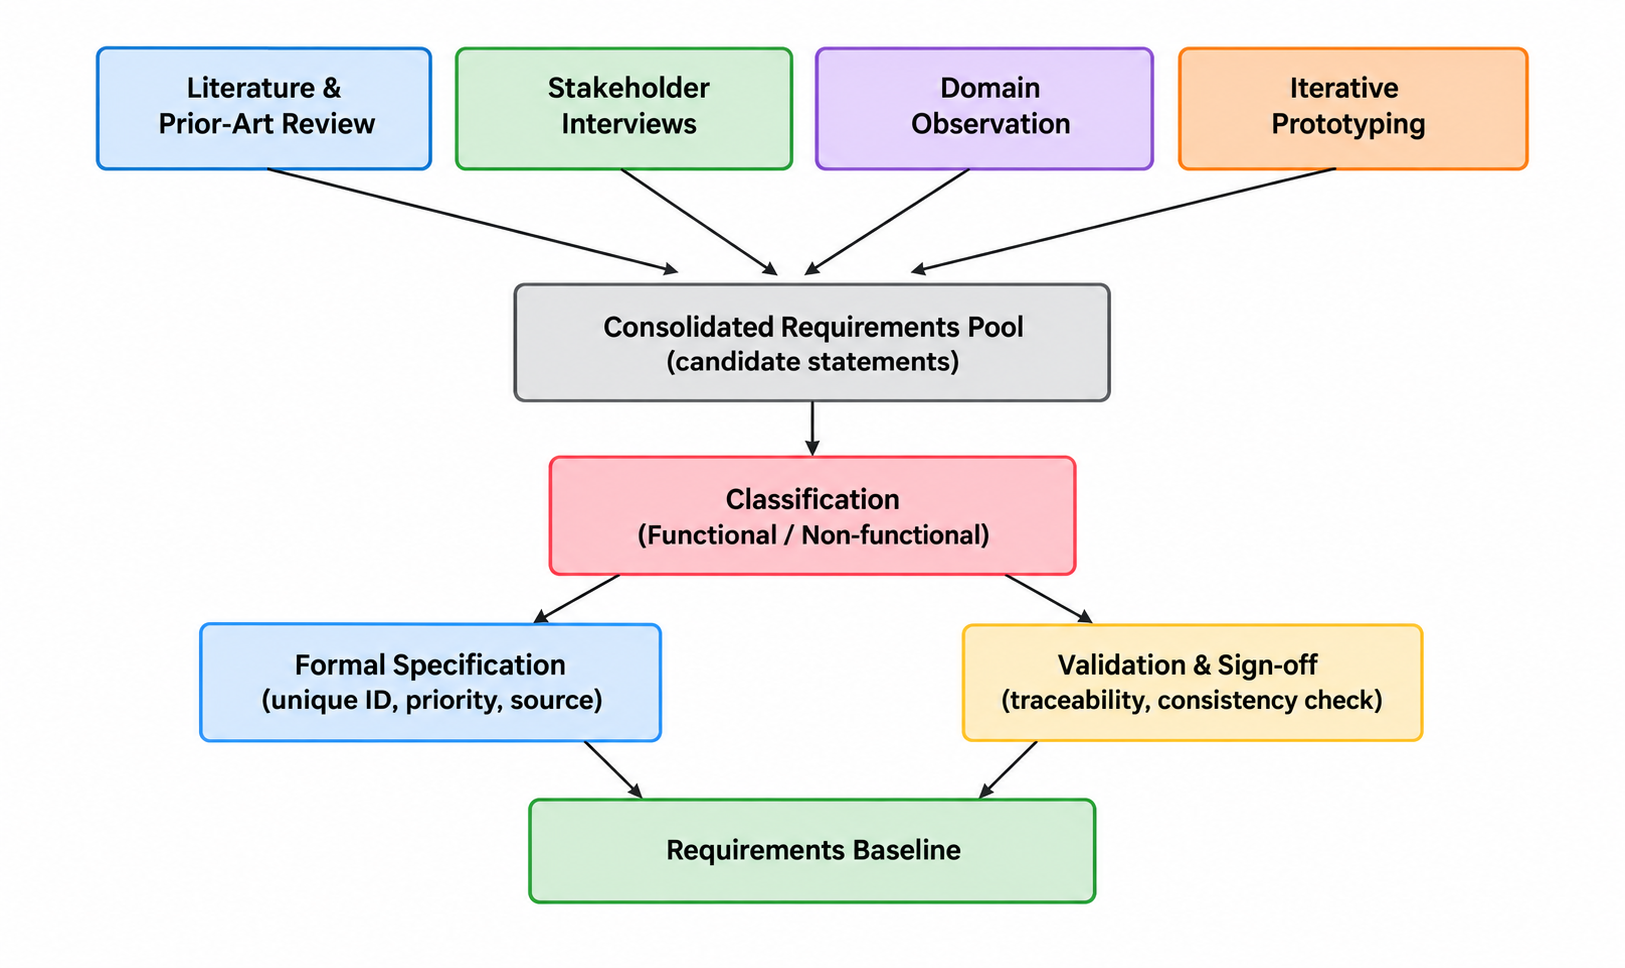
\includegraphics[width=0.92\textwidth]{./../images/requirements/elicitation_process.png}
    \caption{Requirements elicitation and documentation process}
    \label{fig:elicitation}
\end{figure}

The requirements were identified through the following activities:

\begin{itemize}

    \item \textbf{Existing Work Analysis:} Existing revealed two types of approaches for automated crowd counting: detection based (sparse) and density regression (dense). Survey of existing crowd counting methods yielded two categories: automated crowd counting based on the detection of individual people (sparse) methods, which are less accurate when the crowd is heavily occluded, and automated crowd counting based on density regression (dense) methods, which are more accurate when the crowd is heavily occluded. The need for a hybrid approach, not a single fixed approach, was directly triggered by this review.

    \item \textbf{Stakeholder Interviews:} To develop practical constraints, practical users of the system (people who would have to monitor crowd levels in a public or semi public space) were consulted informally. The system was to be usable by anyone, not require specialist machine learning knowledge, and required to work from still images as well as short video clips, and the result should be displayed as a number that an operator could check visually against their own perception of crowd density, not trust blindly.

    \item \textbf{Domain Observation:} To come up with the set of requirements, domain observation was used to look at examples of crowd density in the samples and find failure modes of naive counting methods, which were then translated into requirements: double counting from overlapping detections, under counting in dense occlusion, and counting instability across near identical consecutive frames.

    \item \textbf{Iterative Prototyping:} Single strategy prototypes were also developed and tested with sample footage: problems found during testing were incorporated into the requirements as before, and thresholds were adjusted accordingly, the requirements defined in Section~\ref{sec:functional-requirements} for the scene classification and fusion behaviour were confirmed by observing the results of testing the early prototypes. 
    
\end{itemize}

For each elicited requirement, a uniquely identified statement was subsequently written, assigned a priority, and checked for consistency and duplication with the other requirements before being placed in the baseline described in this chapter. Requirements are identified using either \texttt{FR-nn} for functional requirements or \texttt{NFR-nn} for non-functional requirements. This identifier scheme enables all requirements to be traced to the design elements that satisfy them and to the test cases that verify them.

\section{Functional Requirements}
\label{sec:functional-requirements}

Functional requirements define the observable behaviour and capabilities that the system must demonstrate, without regard to how well those capabilities are performed. Tables~\ref{tab:fr01}--\ref{tab:fr02} describe the functional requirements in each of the four functional areas outlined in Figure~\ref{fig:frtree}, providing their identifiers, descriptions, stakeholders, and priorities.

\begin{figure}[H]
    \centering
    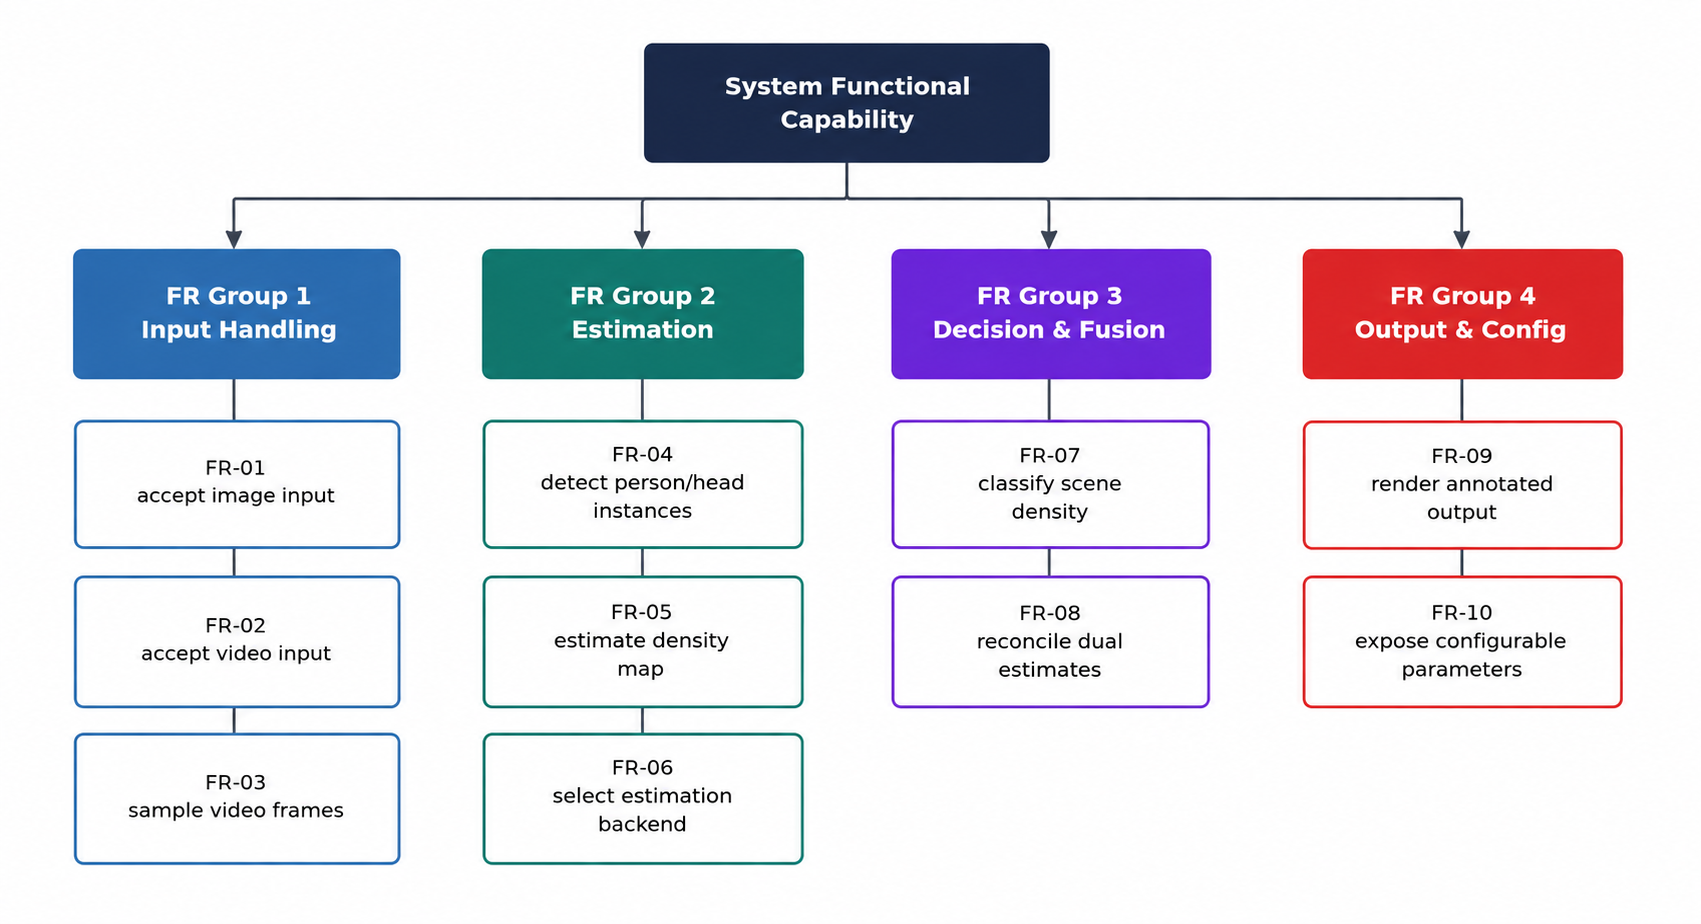
\includegraphics[width=0.95\textwidth]{./../images/requirements/fr_decomposition.png}
    \caption{Overview of functional requirements across different functional groups.}
    \label{fig:frtree}
\end{figure}

% ------------------------------------------------------------
% FR-01: Image Input
% ------------------------------------------------------------

\begin{table}[H]
	\centering
	\renewcommand{\arraystretch}{1.25}
	\begin{tabular}{|p{3.2cm}|p{11.8cm}|}
		\hline
		\textbf{FR-01} &
		\textbf{Image Input} \\ \hline
		
		\textbf{Description} &
		The system shall accept a single still image as an input for crowd estimation. \\ \hline
		
		\multicolumn{2}{|l|}{
			\begin{tabular}{p{3cm}|p{3.5cm}|p{3.5cm}|p{3.5cm}}
				\textbf{Stakeholders:} & Inspector &
				\textbf{Priority:} & High
			\end{tabular}
		} \\ \hline
	\end{tabular}
	\caption{Functional requirement for image input.}
	\label{tab:fr01}
\end{table}

% ------------------------------------------------------------
% FR-02: Video Input
% ------------------------------------------------------------

\begin{table}[H]
	\centering
	\renewcommand{\arraystretch}{1.25}
	\begin{tabular}{|p{3.2cm}|p{11.8cm}|}
		\hline
		\textbf{FR-02} &
		\textbf{Video Input} \\ \hline
		
		\textbf{Description} &
		The system shall accept a video file as an input for frame-based crowd estimation. \\ \hline
		
		\multicolumn{2}{|l|}{
			\begin{tabular}{p{3cm}|p{3.5cm}|p{3.5cm}|p{3.5cm}}
				\textbf{Stakeholders:} & Inspector &
				\textbf{Priority:} & High
			\end{tabular}
		} \\ \hline
	\end{tabular}
	\caption{Functional requirement for video input.}
	\label{tab:fr02}
\end{table}

% ------------------------------------------------------------
% FR-03: Configurable Frame Sampling
% ------------------------------------------------------------

\begin{table}[H]
	\centering
	\renewcommand{\arraystretch}{1.25}
	\begin{tabular}{|p{3.2cm}|p{11.8cm}|}
		\hline
		\textbf{FR-03} &
		\textbf{Configurable Frame Sampling} \\ \hline
		
		\textbf{Description} &
		The system shall sample frames from a video input at a configurable rate rather than processing every frame. The sampling rate shall be adjustable according to the operating requirements of the system. \\ \hline
		
		\multicolumn{2}{|l|}{
			\begin{tabular}{p{3cm}|p{3.5cm}|p{3.5cm}|p{3.5cm}}
				\textbf{Stakeholders:} & Inspector &
				\textbf{Priority:} & Medium
			\end{tabular}
		} \\ \hline
	\end{tabular}
	\caption{Functional requirement for configurable frame sampling.}
	\label{tab:fr03}
\end{table}

% ------------------------------------------------------------
% FR-04: Person/Head Detection
% ------------------------------------------------------------

\begin{table}[H]
	\centering
	\renewcommand{\arraystretch}{1.25}
	\begin{tabular}{|p{3.2cm}|p{11.8cm}|}
		\hline
		\textbf{FR-04} &
		\textbf{Person/Head Detection} \\ \hline
		
		\textbf{Description} &
		The system shall detect discrete person or head instances within a processed frame and report their corresponding locations and total number of detected instances. \\ \hline
		
		\multicolumn{2}{|l|}{
			\begin{tabular}{p{3cm}|p{3.5cm}|p{3.5cm}|p{3.5cm}}
				\textbf{Stakeholders:} & Inspector &
				\textbf{Priority:} & High
			\end{tabular}
		} \\ \hline
	\end{tabular}
	\caption{Functional requirement for person or head detection.}
	\label{tab:fr04}
\end{table}

% ------------------------------------------------------------
% FR-05: Density Map Estimation
% ------------------------------------------------------------

\begin{table}[H]
	\centering
	\renewcommand{\arraystretch}{1.25}
	\begin{tabular}{|p{3.2cm}|p{11.8cm}|}
		\hline
		\textbf{FR-05} &
		\textbf{Density Map Estimation} \\ \hline
		
		\textbf{Description} &
		The system shall estimate a continuous crowd density map for each processed frame and integrate the predicted density map to obtain an estimated crowd count. \\ \hline
		
		\multicolumn{2}{|l|}{
			\begin{tabular}{p{3cm}|p{3.5cm}|p{3.5cm}|p{3.5cm}}
				\textbf{Stakeholders:} & Inspector &
				\textbf{Priority:} & High
			\end{tabular}
		} \\ \hline
	\end{tabular}
	\caption{Functional requirement for density map estimation.}
	\label{tab:fr05}
\end{table}

% ------------------------------------------------------------
% FR-06: Independent Backend Selection
% ------------------------------------------------------------

\begin{table}[H]
	\centering
	\renewcommand{\arraystretch}{1.25}
	\begin{tabular}{|p{3.2cm}|p{11.8cm}|}
		\hline
		\textbf{FR-06} &
		\textbf{Independent Backend Selection} \\ \hline
		
		\textbf{Description} &
		The system shall allow the detection backend and density estimation backend to be selected independently of one another, enabling different combinations of detection and density estimation models to be configured. \\ \hline
		
		\multicolumn{2}{|l|}{
			\begin{tabular}{p{3cm}|p{3.5cm}|p{3.5cm}|p{3.5cm}}
				\textbf{Stakeholders:} & Inspector &
				\textbf{Priority:} & Medium
			\end{tabular}
		} \\ \hline
	\end{tabular}
	\caption{Functional requirement for independent backend selection.}
	\label{tab:fr06}
\end{table}

% ------------------------------------------------------------
% FR-07: Density Classification
% ------------------------------------------------------------

\begin{table}[H]
	\centering
	\renewcommand{\arraystretch}{1.25}
	\begin{tabular}{|p{3.2cm}|p{11.8cm}|}
		\hline
		\textbf{FR-07} &
		\textbf{Density Classification} \\ \hline
		
		\textbf{Description} &
		The system shall classify each processed frame as sparse or dense based on the number of detections observed in the frame. The classification shall determine the appropriate estimation approach for the subsequent processing stage. \\ \hline
		
		\multicolumn{2}{|l|}{
			\begin{tabular}{p{3cm}|p{3.5cm}|p{3.5cm}|p{3.5cm}}
				\textbf{Stakeholders:} & Inspector &
				\textbf{Priority:} & High
			\end{tabular}
		} \\ \hline
	\end{tabular}
	\caption{Functional requirement for density classification.}
	\label{tab:fr07}
\end{table}

% ------------------------------------------------------------
% FR-08: Estimate Fusion
% ------------------------------------------------------------

\begin{table}[H]
	\centering
	\renewcommand{\arraystretch}{1.25}
	\begin{tabular}{|p{3.2cm}|p{11.8cm}|}
		\hline
		\textbf{FR-08} &
		\textbf{Detection and Density Estimate Fusion} \\ \hline
		
		\textbf{Description} &
		The system shall combine the detection based and density based crowd estimates to produce a single final crowd estimate for each processed frame. \\ \hline
		
		\multicolumn{2}{|l|}{
			\begin{tabular}{p{3cm}|p{3.5cm}|p{3.5cm}|p{3.5cm}}
				\textbf{Stakeholders:} & Inspector &
				\textbf{Priority:} & High
			\end{tabular}
		} \\ \hline
	\end{tabular}
	\caption{Functional requirement for detection and density estimate fusion.}
	\label{tab:fr08}
\end{table}

% ------------------------------------------------------------
% FR-09: Annotated Output
% ------------------------------------------------------------

\begin{table}[H]
	\centering
	\renewcommand{\arraystretch}{1.25}
	\begin{tabular}{|p{3.2cm}|p{11.8cm}|}
		\hline
		\textbf{FR-09} &
		\textbf{Annotated Output} \\ \hline
		
		\textbf{Description} &
		The system shall display an annotated image or video containing the estimated number of detected instances for the corresponding input. \\ \hline
		
		\multicolumn{2}{|l|}{
			\begin{tabular}{p{3cm}|p{3.5cm}|p{3.5cm}|p{3.5cm}}
				\textbf{Stakeholders:} & Inspector &
				\textbf{Priority:} & High
			\end{tabular}
		} \\ \hline
	\end{tabular}
	\caption{Functional requirement for annotated output.}
	\label{tab:fr09}
\end{table}

% ------------------------------------------------------------
% FR-10: External Configuration
% ------------------------------------------------------------

\begin{table}[H]
	\centering
	\renewcommand{\arraystretch}{1.25}
	\begin{tabular}{|p{3.2cm}|p{11.8cm}|}
		\hline
		\textbf{FR-10} &
		\textbf{External Configuration} \\ \hline
		
		\textbf{Description} &
		The system shall expose its operating parameters through an externally editable configuration file. The configuration shall include parameters such as the density threshold, detection and density estimation backend selection, and video frame sampling rate. \\ \hline
		
		\multicolumn{2}{|l|}{
			\begin{tabular}{p{3cm}|p{3.5cm}|p{3.5cm}|p{3.5cm}}
				\textbf{Stakeholders:} & Inspector &
				\textbf{Priority:} & Medium
			\end{tabular}
		} \\ \hline
	\end{tabular}
	\caption{Functional requirement for external system configuration.}
	\label{tab:fr10}
\end{table}

\section{Non-functional Requirements}
\label{sec:nfr}

Non-functional requirements constrain how the system operates and specify quality characteristics such as performance, robustness, user-friendliness, maintainability, and security. The relative importance of each characteristic for this system is shown in Figure~\ref{fig:nfrradar}, and the individual requirements are documented in Tables~\ref{tab:nfr01}--\ref{tab:nfr08}.

\begin{figure}[H]
    \centering
    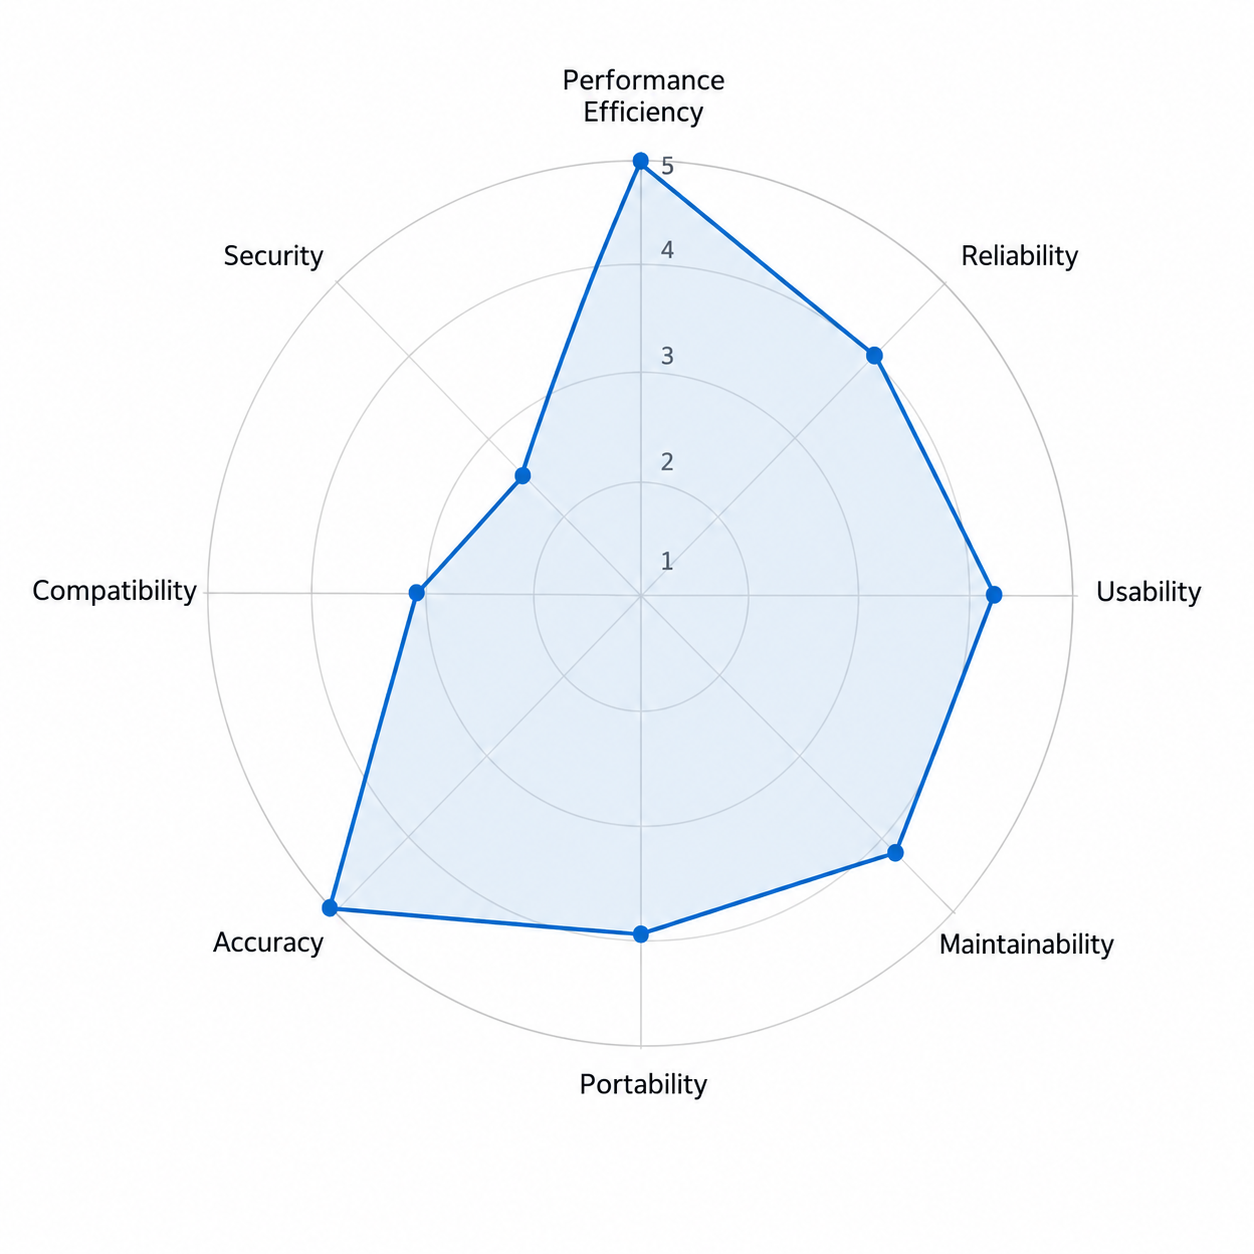
\includegraphics[width=0.62\textwidth]{./../images/requirements/nfr_radar.png}
    \caption{Quality characteristics of NFR with the relative emphasis}
    \label{fig:nfrradar}
\end{figure}

The accuracy and performance efficiency dominate the profile in Figure~\ref{fig:nfrradar}, as the main value proposition of the system is delivering an accurate and reliable numerical estimate within a practically useful time budget. Usability is given a high weight because the intended operator is not assumed to have machine learning expertise. Security is comparatively low because of the current deployment model of the system, in which it is operated by one person and runs offline.

% ------------------------------------------------------------
% NFR-01: Performance Efficiency
% ------------------------------------------------------------

\begin{table}[H]
	\centering
	\renewcommand{\arraystretch}{1.25}
	\begin{tabular}{|p{3.2cm}|p{11.8cm}|}
		\hline
		\textbf{NFR-01} &
		\textbf{Performance Efficiency} \\ \hline
		
		\textbf{Description} &
		The system shall process a single input frame within a bounded and predefined time when executed on commodity computing hardware. The processing time shall remain sufficiently low to support practical frame based crowd estimation. \\ \hline
		
		\multicolumn{2}{|l|}{
			\begin{tabular}{p{3cm}|p{3.5cm}|p{3.5cm}|p{3.5cm}}
				\textbf{Stakeholders:} & Inspector &
				\textbf{Priority:} & High
			\end{tabular}
		} \\ \hline
	\end{tabular}
	\caption{Non-functional requirement for performance efficiency.}
	\label{tab:nfr01}
\end{table}

% ------------------------------------------------------------
% NFR-02: Accuracy
% ------------------------------------------------------------

\begin{table}[H]
	\centering
	\renewcommand{\arraystretch}{1.25}
	\begin{tabular}{|p{3.2cm}|p{11.8cm}|}
		\hline
		\textbf{NFR-02} &
		\textbf{Accuracy} \\ \hline
		
		\textbf{Description} &
		The fused crowd estimate shall maintain an acceptable level of agreement with the ground truth count across both sparse and dense scenes. The system shall be evaluated using appropriate crowd counting performance metrics to assess its estimation accuracy. \\ \hline
		
		\multicolumn{2}{|l|}{
			\begin{tabular}{p{3cm}|p{3.5cm}|p{3.5cm}|p{3.5cm}}
				\textbf{Stakeholders:} & Inspector &
				\textbf{Priority:} & High
			\end{tabular}
		} \\ \hline
	\end{tabular}
	\caption{Non-functional requirement for crowd counting accuracy.}
	\label{tab:nfr02}
\end{table}

% ------------------------------------------------------------
% NFR-03: Reliability
% ------------------------------------------------------------

\begin{table}[H]
	\centering
	\renewcommand{\arraystretch}{1.25}
	\begin{tabular}{|p{3.2cm}|p{11.8cm}|}
		\hline
		\textbf{NFR-03} &
		\textbf{Reliability} \\ \hline
		
		\textbf{Description} &
		The system shall be capable of processing a complete video without unexpected termination or system crashes caused by malformed, corrupted, empty, or otherwise invalid frames encountered during processing. \\ \hline
		
		\multicolumn{2}{|l|}{
			\begin{tabular}{p{3cm}|p{3.5cm}|p{3.5cm}|p{3.5cm}}
				\textbf{Stakeholders:} & Inspector &
				\textbf{Priority:} & High
			\end{tabular}
		} \\ \hline
	\end{tabular}
	\caption{Non-functional requirement for system reliability.}
	\label{tab:nfr03}
\end{table}

% ------------------------------------------------------------
% NFR-04: Usability
% ------------------------------------------------------------

\begin{table}[H]
	\centering
	\renewcommand{\arraystretch}{1.25}
	\begin{tabular}{|p{3.2cm}|p{11.8cm}|}
		\hline
		\textbf{NFR-04} &
		\textbf{Usability} \\ \hline
		
		\textbf{Description} &
		The system shall provide a sufficiently straightforward execution and configuration process such that an operator without detailed knowledge of the system's internal implementation can run the crowd estimation pipeline without external assistance. \\ \hline
		
		\multicolumn{2}{|l|}{
			\begin{tabular}{p{3cm}|p{3.5cm}|p{3.5cm}|p{3.5cm}}
				\textbf{Stakeholders:} & Inspector &
				\textbf{Priority:} & Medium
			\end{tabular}
		} \\ \hline
	\end{tabular}
	\caption{Non-functional requirement for system usability.}
	\label{tab:nfr04}
\end{table}

% ------------------------------------------------------------
% NFR-05: Maintainability
% ------------------------------------------------------------

\begin{table}[H]
	\centering
	\renewcommand{\arraystretch}{1.25}
	\begin{tabular}{|p{3.2cm}|p{11.8cm}|}
		\hline
		\textbf{NFR-05} &
		\textbf{Maintainability} \\ \hline
		
		\textbf{Description} &
		The system shall employ a modular architecture in which individual detection and density estimation backends can be replaced, updated, or modified without requiring changes to unrelated modules of the processing pipeline. \\ \hline
		
		\multicolumn{2}{|l|}{
			\begin{tabular}{p{3cm}|p{3.5cm}|p{3.5cm}|p{3.5cm}}
				\textbf{Stakeholders:} & Developer, Inspector &
				\textbf{Priority:} & High
			\end{tabular}
		} \\ \hline
	\end{tabular}
	\caption{Non-functional requirement for system maintainability.}
	\label{tab:nfr05}
\end{table}

% ------------------------------------------------------------
% NFR-06: Portability
% ------------------------------------------------------------

\begin{table}[H]
	\centering
	\renewcommand{\arraystretch}{1.25}
	\begin{tabular}{|p{3.2cm}|p{11.8cm}|}
		\hline
		\textbf{NFR-06} &
		\textbf{Portability} \\ \hline
		
		\textbf{Description} &
		The system shall be executable without modification on the major desktop operating systems supported by the underlying runtime environment, provided that the required dependencies and execution environment are available. \\ \hline
		
		\multicolumn{2}{|l|}{
			\begin{tabular}{p{3cm}|p{3.5cm}|p{3.5cm}|p{3.5cm}}
				\textbf{Stakeholders:} & Developer, Inspector &
				\textbf{Priority:} & Medium
			\end{tabular}
		} \\ \hline
	\end{tabular}
	\caption{Non-functional requirement for system portability.}
	\label{tab:nfr06}
\end{table}

% ------------------------------------------------------------
% NFR-07: Compatibility
% ------------------------------------------------------------

\begin{table}[H]
	\centering
	\renewcommand{\arraystretch}{1.25}
	\begin{tabular}{|p{3.2cm}|p{11.8cm}|}
		\hline
		\textbf{NFR-07} &
		\textbf{Input Compatibility} \\ \hline
		
		\textbf{Description} &
		The system shall support commonly used image and video file formats without requiring the input files to be manually converted into another format before processing. \\ \hline
		
		\multicolumn{2}{|l|}{
			\begin{tabular}{p{3cm}|p{3.5cm}|p{3.5cm}|p{3.5cm}}
				\textbf{Stakeholders:} & Inspector &
				\textbf{Priority:} & Medium
			\end{tabular}
		} \\ \hline
	\end{tabular}
	\caption{Non-functional requirement for input compatibility.}
	\label{tab:nfr07}
\end{table}

% ------------------------------------------------------------
% NFR-08: Input and Asset Validation
% ------------------------------------------------------------

\begin{table}[H]
	\centering
	\renewcommand{\arraystretch}{1.25}
	\begin{tabular}{|p{3.2cm}|p{11.8cm}|}
		\hline
		\textbf{NFR-08} &
		\textbf{Input and Asset Validation} \\ \hline
		
		\textbf{Description} &
		The system shall validate input files and required model assets before initiating the estimation process. Invalid, inaccessible, corrupted, or incompatible inputs and model assets shall be identified and handled without causing unexpected system failure. \\ \hline
		
		\multicolumn{2}{|l|}{
			\begin{tabular}{p{3cm}|p{3.5cm}|p{3.5cm}|p{3.5cm}}
				\textbf{Stakeholders:} & Developer, Inspector &
				\textbf{Priority:} & High
			\end{tabular}
		} \\ \hline
	\end{tabular}
	\caption{Non-functional requirement for input and model asset validation.}
	\label{tab:nfr08}
\end{table}

\section{Use Cases and Scenarios}

This section states the functional requirements of Section~\ref{sec:functional-requirements} from the perspective of the actor who interacts with the system. The overall use-case diagram is displayed in Figure~\ref{fig:usecase} and shows the sole actor, the \emph{Operator}, together with the five use cases described below.

\begin{figure}[H]
    \centering
    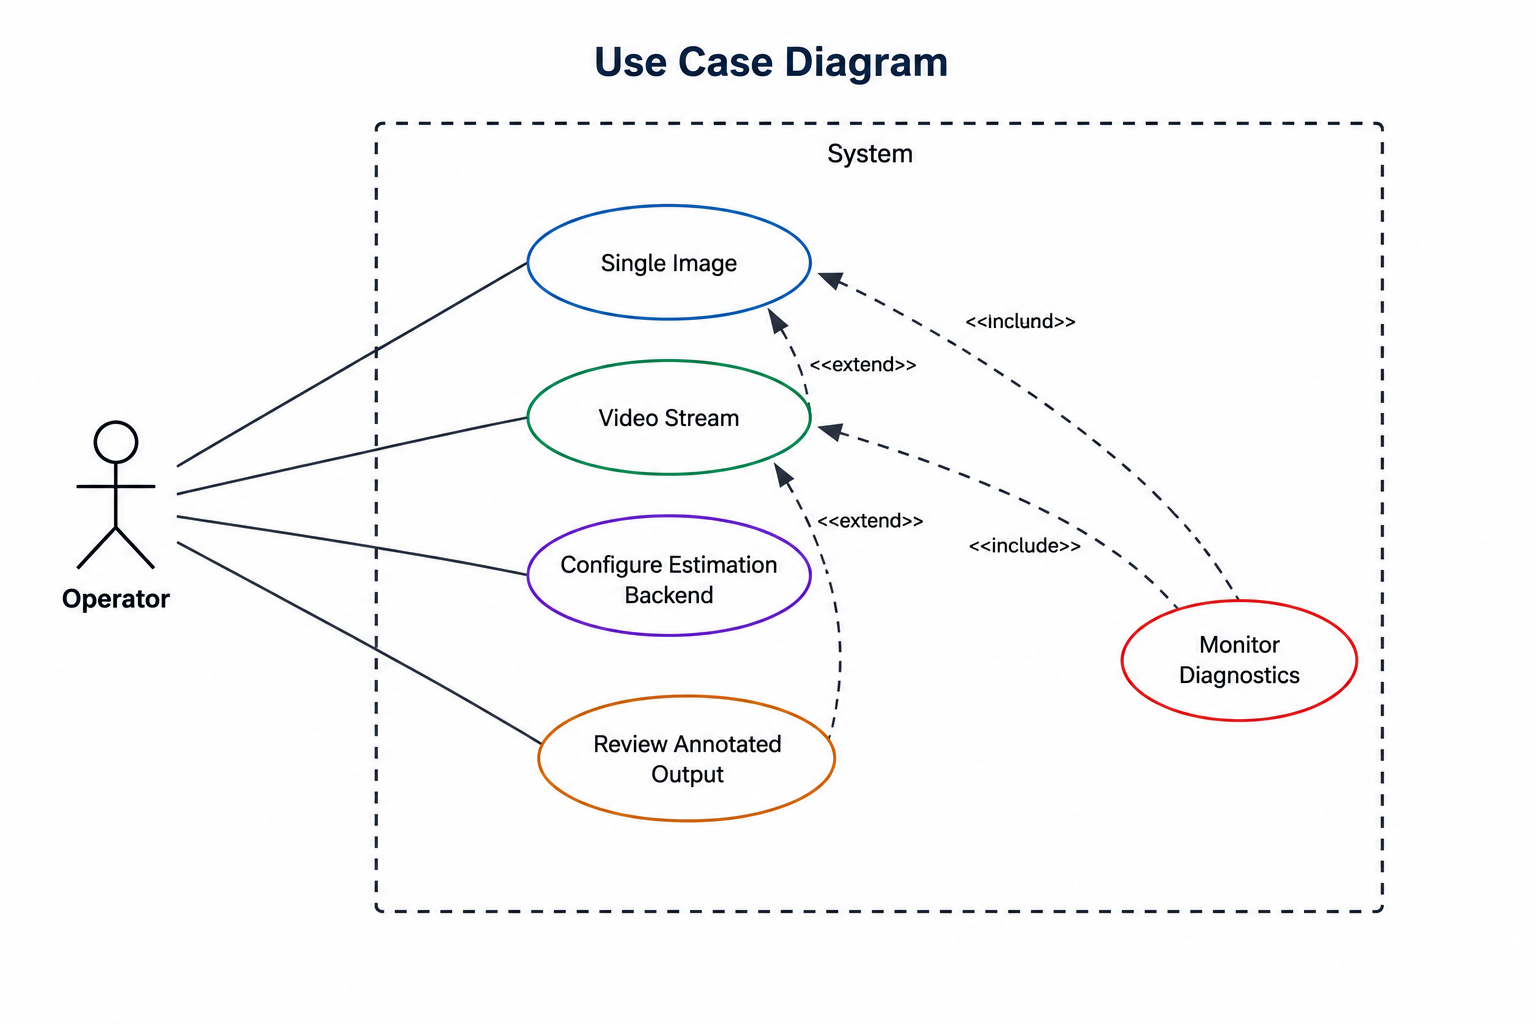
\includegraphics[width=\textwidth]{./../images/requirements/use_case_diagram.png}
    \caption{Use case diagram}
    \label{fig:usecase}
\end{figure}

% ============================================================
% Use Case 1
% ============================================================

The first use case covers the simplest interaction with the system: submitting one still image and receiving a single fused count in return.

\begin{longtable}{|
    >{\raggedright\arraybackslash}p{3.0cm}|
    >{\raggedright\arraybackslash}p{\dimexpr\textwidth-3.0cm-4\tabcolsep-3\arrayrulewidth\relax}|
}
\caption{UC-1: Single Image}
\label{tab:uc1} \\

\hline
\textbf{Field} & \textbf{Description} \\
\hline
\endfirsthead

\hline
\textbf{Field} & \textbf{Description} \\
\hline
\endhead

\textbf{Identifier} &
UC-1
\\
\hline

\textbf{Actor(s)} &
Operator (primary)
\\
\hline

\textbf{Related requirements} &
FR-01, FR-04, FR-05, FR-07, FR-08, FR-09
\\
\hline

\textbf{Preconditions} &
The system has been started and the necessary model assets are available. The operator has an image file capable of being read.
\\
\hline

\textbf{Main flow} &
\begin{itemize}[leftmargin=16pt, itemsep=0pt, topsep=0pt]
    \item The operator sets the image mode and provides the path of an image file.

    \item The system checks the file and reads it into the system.

    \item The system preprocesses the image and performs sparse and dense estimation.

    \item The system categorises the scene, combines the two estimates, and produces a single count.

    \item The system displays an annotated image with detections and a fused count to the operator.
\end{itemize}
\\
\hline

\textbf{Alternative flow} &
If the path provided is not readable or is not a valid image, the system displays an error and asks the operator for a path again.
\\
\hline

\textbf{Postconditions} &
The operator can see an annotated image and has a fused count available. The run is written to the diagnostic log.
\\
\hline

\end{longtable}

% ============================================================
% Use Case 2
% ============================================================

Building on UC-1, the second use case extends the same estimation behaviour from a single frame to an entire video, adding temporal sampling and cross frame identity tracking.

\begin{longtable}{|
    >{\raggedright\arraybackslash}p{3.0cm}|
    >{\raggedright\arraybackslash}p{\dimexpr\textwidth-3.0cm-4\tabcolsep-3\arrayrulewidth\relax}|
}
\caption{UC-2: Video Stream}
\label{tab:uc2} \\

\hline
\textbf{Field} & \textbf{Description} \\
\hline
\endfirsthead

\hline
\textbf{Field} & \textbf{Description} \\
\hline
\endhead

\textbf{Identifier} &
UC-2
\\
\hline

\textbf{Actor(s)} &
Operator (primary)
\\
\hline

\textbf{Related requirements} &
FR-02, FR-03, FR-04, FR-05, FR-07, FR-08, FR-09
\\
\hline

\textbf{Preconditions} &
The system is running and the necessary model resources are available. The operator has a video file to read.
\\
\hline

\textbf{Main flow} &
\begin{itemize}[leftmargin=16pt, itemsep=0pt, topsep=0pt]
    \item The operator selects video mode and provides a video file.

    \item The system validates the file and identifies its native frame rate.

    \item The system samples frames at the configured rate and, for each sampled frame, performs estimation and fusion as described in UC-1.

    \item The system stores detections across sampled frames to maintain the identity of each individual throughout the clip.

    \item The system provides an annotated output video and summary statistics, including the average and maximum number of fused individuals and the total number of unique individuals observed.
\end{itemize}
\\
\hline

\textbf{Alternative flow} &
If the video cannot be opened or contains no readable frames, the system displays an error and asks the operator for a path again.
\\
\hline

\textbf{Postconditions} &
The operator receives an annotated output video and a run summary, and the run is recorded in the diagnostic log.
\\
\hline

\end{longtable}

% ============================================================
% Use Case 3
% ============================================================

Before running UC-1 or UC-2, the operator may first want to choose which estimation strategy the system should use. This configuration step is described next.

\begin{longtable}{|
    >{\raggedright\arraybackslash}p{3.0cm}|
    >{\raggedright\arraybackslash}p{\dimexpr\textwidth-3.0cm-4\tabcolsep-3\arrayrulewidth\relax}|
}
\caption{UC-3: Configure Estimation Backend}
\label{tab:uc3} \\

\hline
\textbf{Field} & \textbf{Description} \\
\hline
\endfirsthead

\hline
\textbf{Field} & \textbf{Description} \\
\hline
\endhead

\textbf{Identifier} &
UC-3
\\
\hline

\textbf{Actor(s)} &
Operator (primary)
\\
\hline

\textbf{Related requirements} &
FR-06, FR-10
\\
\hline

\textbf{Preconditions} &
The operator is able to access and modify the system configuration information.
\\
\hline

\textbf{Main flow} &
\begin{itemize}[leftmargin=16pt, itemsep=0pt, topsep=0pt]
    \item The operator accesses the configuration and selects the appropriate detection backend and/or density estimation backend.

    \item The operator adjusts the associated thresholds, such as confidence thresholds and scene decision thresholds, as necessary.

    \item The system checks whether the supplied configuration values are within their expected ranges.

    \item The new configuration is used for subsequent runs (UC-1 and UC-2).
\end{itemize}
\\
\hline

\textbf{Alternative flow} &
If a supplied parameter is outside its valid range, the system rejects the change and retains the previous value.
\\
\hline

\textbf{Postconditions} &
Subsequent runs use the newly selected backend(s) and configuration parameters.
\\
\hline

\end{longtable}

% ============================================================
% Use Case 4
% ============================================================

Once a run from UC-1 or UC-2 has produced output, the operator typically inspects that output before trusting it. This review step is described next.

\begin{longtable}{|
    >{\raggedright\arraybackslash}p{3.0cm}|
    >{\raggedright\arraybackslash}p{\dimexpr\textwidth-3.0cm-4\tabcolsep-3\arrayrulewidth\relax}|
}
\caption{UC-4: Review Annotated Output}
\label{tab:uc4} \\

\hline
\textbf{Field} & \textbf{Description} \\
\hline
\endfirsthead

\hline
\textbf{Field} & \textbf{Description} \\
\hline
\endhead

\textbf{Identifier} &
UC-4
\\
\hline

\textbf{Actor(s)} &
Operator (primary)
\\
\hline

\textbf{Related requirements} &
FR-09
\\
\hline

\textbf{Preconditions} &
At least one run (UC-1 or UC-2) has been completed and an output artefact has been produced.
\\
\hline

\textbf{Main flow} &
\begin{itemize}[leftmargin=16pt, itemsep=0pt, topsep=0pt]
    \item The operator opens the annotated output artefact from a previous run.

    \item The operator visually checks the drawn detections, scene classification, and fused or unique counts.
\end{itemize}
\\
\hline

\textbf{Extends} &
UC-1, UC-2. This use case can only be reached after output from one of these use cases has been produced.
\\
\hline

\textbf{Postconditions} &
The operator has made a decision regarding the trustworthiness of the result for the given run.
\\
\hline

\end{longtable}

% ============================================================
% Use Case 5
% ============================================================

Independently of reviewing any single run's output, the operator may also need to check the system's overall health and history. This is covered by the final use case.

\begin{longtable}{|
    >{\raggedright\arraybackslash}p{3.0cm}|
    >{\raggedright\arraybackslash}p{\dimexpr\textwidth-3.0cm-4\tabcolsep-3\arrayrulewidth\relax}|
}
\caption{UC-5: Monitor Diagnostics}
\label{tab:uc5} \\

\hline
\textbf{Field} & \textbf{Description} \\
\hline
\endfirsthead

\hline
\textbf{Field} & \textbf{Description} \\
\hline
\endhead

\textbf{Identifier} &
UC-5
\\
\hline

\textbf{Actor(s)} &
Operator (primary)
\\
\hline

\textbf{Related requirements} &
NFR-01, NFR-03
\\
\hline

\textbf{Preconditions} &
A run (UC-1 or UC-2) is in progress or has been completed.
\\
\hline

\textbf{Main flow} &
\begin{itemize}[leftmargin=16pt, itemsep=0pt, topsep=0pt]
    \item A start event, end event, and elapsed time are automatically recorded for each processing step during every run.

    \item If the system encounters a failure, it records diagnostic details and identifies the failed stage rather than failing silently.

    \item The operator reviews the recorded log to verify normal operation or identify faulty conditions.
\end{itemize}
\\
\hline

\textbf{Includes} &
UC-1, UC-2. Diagnostic recording is automatically included in every run.
\\
\hline

\textbf{Postconditions} &
A detailed diagnostic report of the run is produced and can be reviewed at any time in the future.
\\
\hline

\end{longtable}